\documentclass[11pt]{article}

\usepackage[margin=1in]{geometry}
\usepackage{amsmath,amssymb,bm}
\usepackage{booktabs}
\usepackage{array}
\usepackage{enumitem}
\usepackage{graphicx}
\usepackage{microtype}
\usepackage{placeins}
\usepackage[hidelinks]{hyperref}

\graphicspath{{figures/}}

\newcommand{\vect}[1]{\bm{#1}}
\newcommand{\mat}[1]{\mathbf{#1}}
\newcommand{\norm}[1]{\left\lVert #1 \right\rVert}
\newcommand{\code}[1]{\texttt{#1}}
\DeclareMathOperator*{\argmin}{arg\,min}
\DeclareMathOperator{\logit}{logit}
\DeclareMathOperator{\diag}{diag}

\title{Linking Bounded Single-Epoch Coupling Estimates\\with Structured Priors from a Known Earthquake Time}
\author{Brendan J. Meade}
\date{September 2026 \\[2pt] \small Working document; companion to \code{toy\_method1\_posthoc\_fusion.py}}

\begin{document}
\maketitle

\begin{abstract}
\noindent
Bounded kinematic block models estimated independently at many epochs cannot simply be smoothed in time: each bounded estimate is the mode of a truncated distribution, and averaging such modes biases locked patches away from the bound. This note describes a post-hoc linking method that combines the independent bounded epoch solutions using prior information that is actually known in practice. The earthquake time is known, so the block rate is piecewise constant between earthquakes and the temporal prior breaks only at the earthquake. Where the prescribed bounds admit afterslip, postseismic coupling recovers monotonically and smoothly in log time. Epochs pinned at a bound are treated as censored observations rather than exact ones. On a two-dimensional antiplane toy with two slow slip events, an earthquake, and afterslip, the method recovers the block rate eight times more accurately than the per-epoch solves, reproduces the locked patch exactly, tracks the postseismic recovery to within about 0.1 in coupling, and preserves the pre-earthquake transients. It uses only the per-epoch bounded point estimates, their active constraint sets, and the sufficient statistics of each epoch.
\end{abstract}

\section{Setting}

At each epoch $t$ a bounded solve returns a state vector $\vect{x}_t^\ast$ and the set of coupling bounds that were active at the optimum. For the toy the state is
\begin{equation}
\vect{x}_t = [\,v_0,\; e_1,\; e_2\,]_t,
\end{equation}
the block rate and the elastic slip-deficit rates on two fault patches, and the coupling on patch $i$ is $\kappa_i = e_i / v_0$. Known per-epoch bounds $\kappa_{\mathrm{lo},i}(t) \le \kappa_i(t) \le \kappa_{\mathrm{hi},i}(t)$ are enforced at every epoch on every patch. The bounded solve at epoch $t$ is
\begin{equation}
\vect{x}_t^\ast = \argmin_{\vect{x}}\; \norm{\mat{W}_t^{1/2}(\mat{A}\vect{x} - \vect{d}_t)}^2
\quad\text{s.t.}\quad v_0 \ge 0,\;\; \kappa_{\mathrm{lo},i}(t)\, v_0 \le e_i \le \kappa_{\mathrm{hi},i}(t)\, v_0,
\label{eq:epoch}
\end{equation}
where $\vect{d}_t$ is the epoch velocity field and $\mat{W}_t$ its diagonal weight. Because the sign of $v_0$ is known, the coupling constraint is linear in the joint state and \eqref{eq:epoch} is a small convex quadratic program. In the toy it is solved exactly by enumerating active sets; in \code{celeri} it stands for whatever bounded per-epoch solver is in use. Only three things from each epoch are used downstream: the point estimate $\vect{x}_t^\ast$, the active set, and the sufficient statistics $\mat{H}_t = \mat{A}^{\!\top}\mat{W}_t\mat{A}$ and $\vect{g}_t = \mat{A}^{\!\top}\mat{W}_t\vect{d}_t$.

Two facts about $\vect{x}_t^\ast$ shape the method. First, on a patch whose bound is active the estimate sits exactly on the bound, and the covariance of the constrained estimator has zero width normal to it. The reduced covariance
\begin{equation}
\mat{\Sigma}_t = \mat{N}\bigl(\mat{N}^{\!\top}\mat{H}_t\mat{N}\bigr)^{-1}\mat{N}^{\!\top},
\qquad \mat{N} = \text{null space of the active constraint rows},
\label{eq:reduced}
\end{equation}
captures this. Second, and less obviously, \eqref{eq:reduced} describes the estimator, not our knowledge of the truth: a pinned epoch says that the unconstrained estimate lay at or beyond the bound, which is a one-sided, censored observation with the unconstrained variance, not an exact one. Section~\ref{sec:priors} uses both readings, each where it is appropriate.

\section{The toy}

Figure~\ref{fig:forward} shows the forward model, taken from the Kalman and IMM prototype notebooks with parameter changes noted in the script. A vertical strike-slip fault is locked from 0 to 30 km and split into a shallow patch (0 to 15 km) and a deep patch (15 to 30 km); the fault creeps at the block rate below 30 km. Surface velocities at 50 stations spanning $\pm 150$ km follow the antiplane screw-dislocation solution. The block rate is $0.5$ before an earthquake at $t = 0.5$ and $0.25$ after. The shallow patch hosts a slow slip event at $t = 0.35$ (peak slip rate six times the plate rate) and the coseismic step; the deep patch hosts a slow slip event at $t = 0.25$ (peak twice the plate rate) and exponential afterslip after the earthquake with an initial rate eight times the post-earthquake plate rate. Positions are the time integral of velocity plus the coseismic step plus white noise.

The record is cut into 40 non-overlapping epochs with a boundary exactly at the earthquake. Each epoch's velocity field is the least-squares slope of position against time, with the analytic slope variance. The known bounds are $\kappa \in [-10, 1]$ on both patches before the earthquake; afterwards $[0, 1]$ on the shallow patch and $[-20, 1]$ on the deep patch, tightened to $[-5, 1]$ at $t = 0.75$. Bounds are compared against the epoch-mean truth $\kappa_i = 1 - \bar{s}_i / \bar{v}_0$.

\begin{figure}[htbp]
\centering
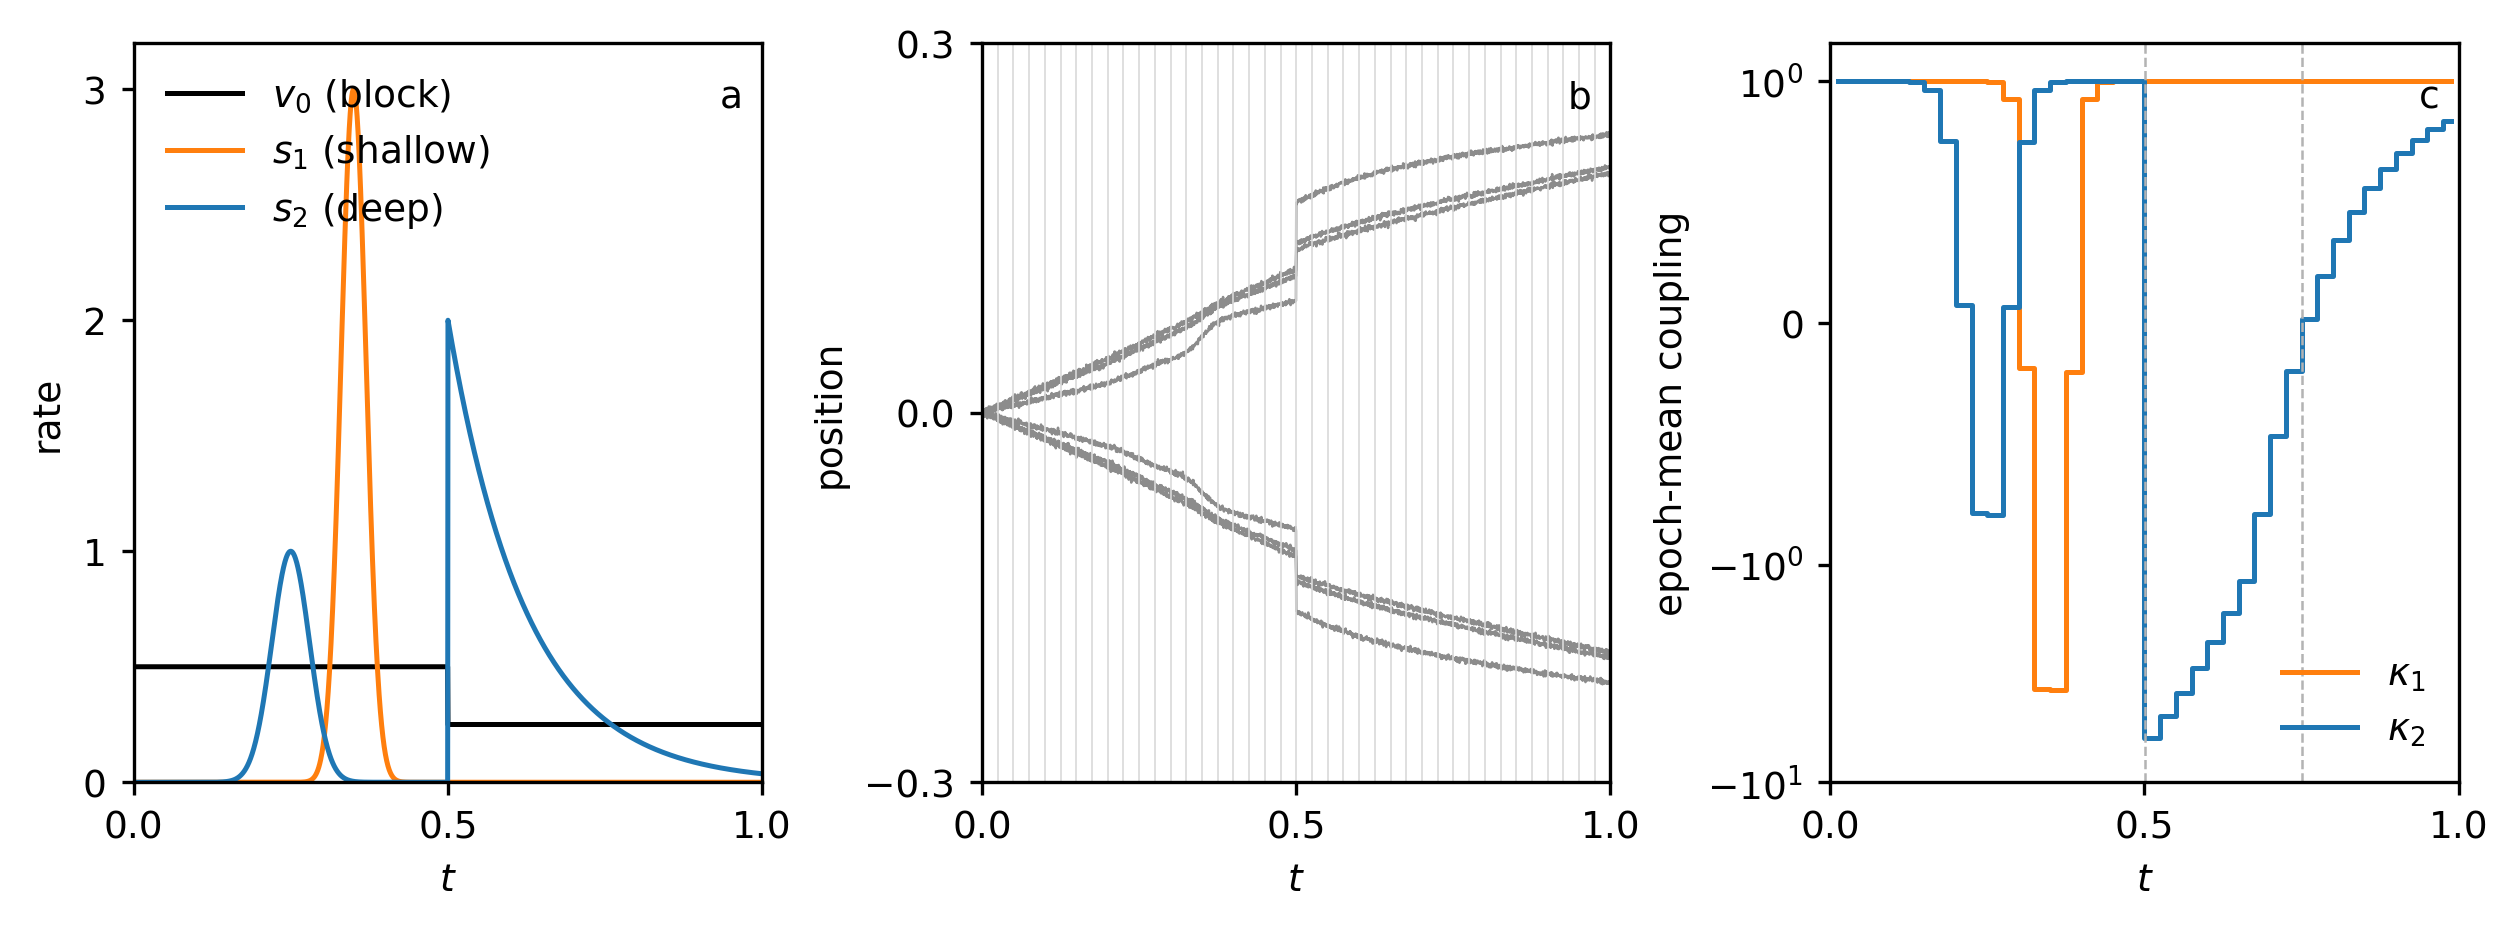
\includegraphics[width=\textwidth]{fig1_forward_model.png}
\caption{Forward model. (a) Truth histories of the block rate $v_0$ and the patch slip rates $s_1$, $s_2$. (b) Noisy positions at six stations; vertical lines are epoch boundaries. (c) Epoch-mean truth coupling on the two patches on a symmetric-log axis.}
\label{fig:forward}
\end{figure}

Figure~\ref{fig:epochs} shows the independent per-epoch solves. The unconstrained estimates scatter above and below 1 on locked patches; the bounded estimates are one-sided, half pinned at exactly 1 and half below. Their mean on the locked shallow patch after the earthquake is 0.948 against a truth of 1. This is the bias that any naive smoother inherits.

\begin{figure}[htbp]
\centering
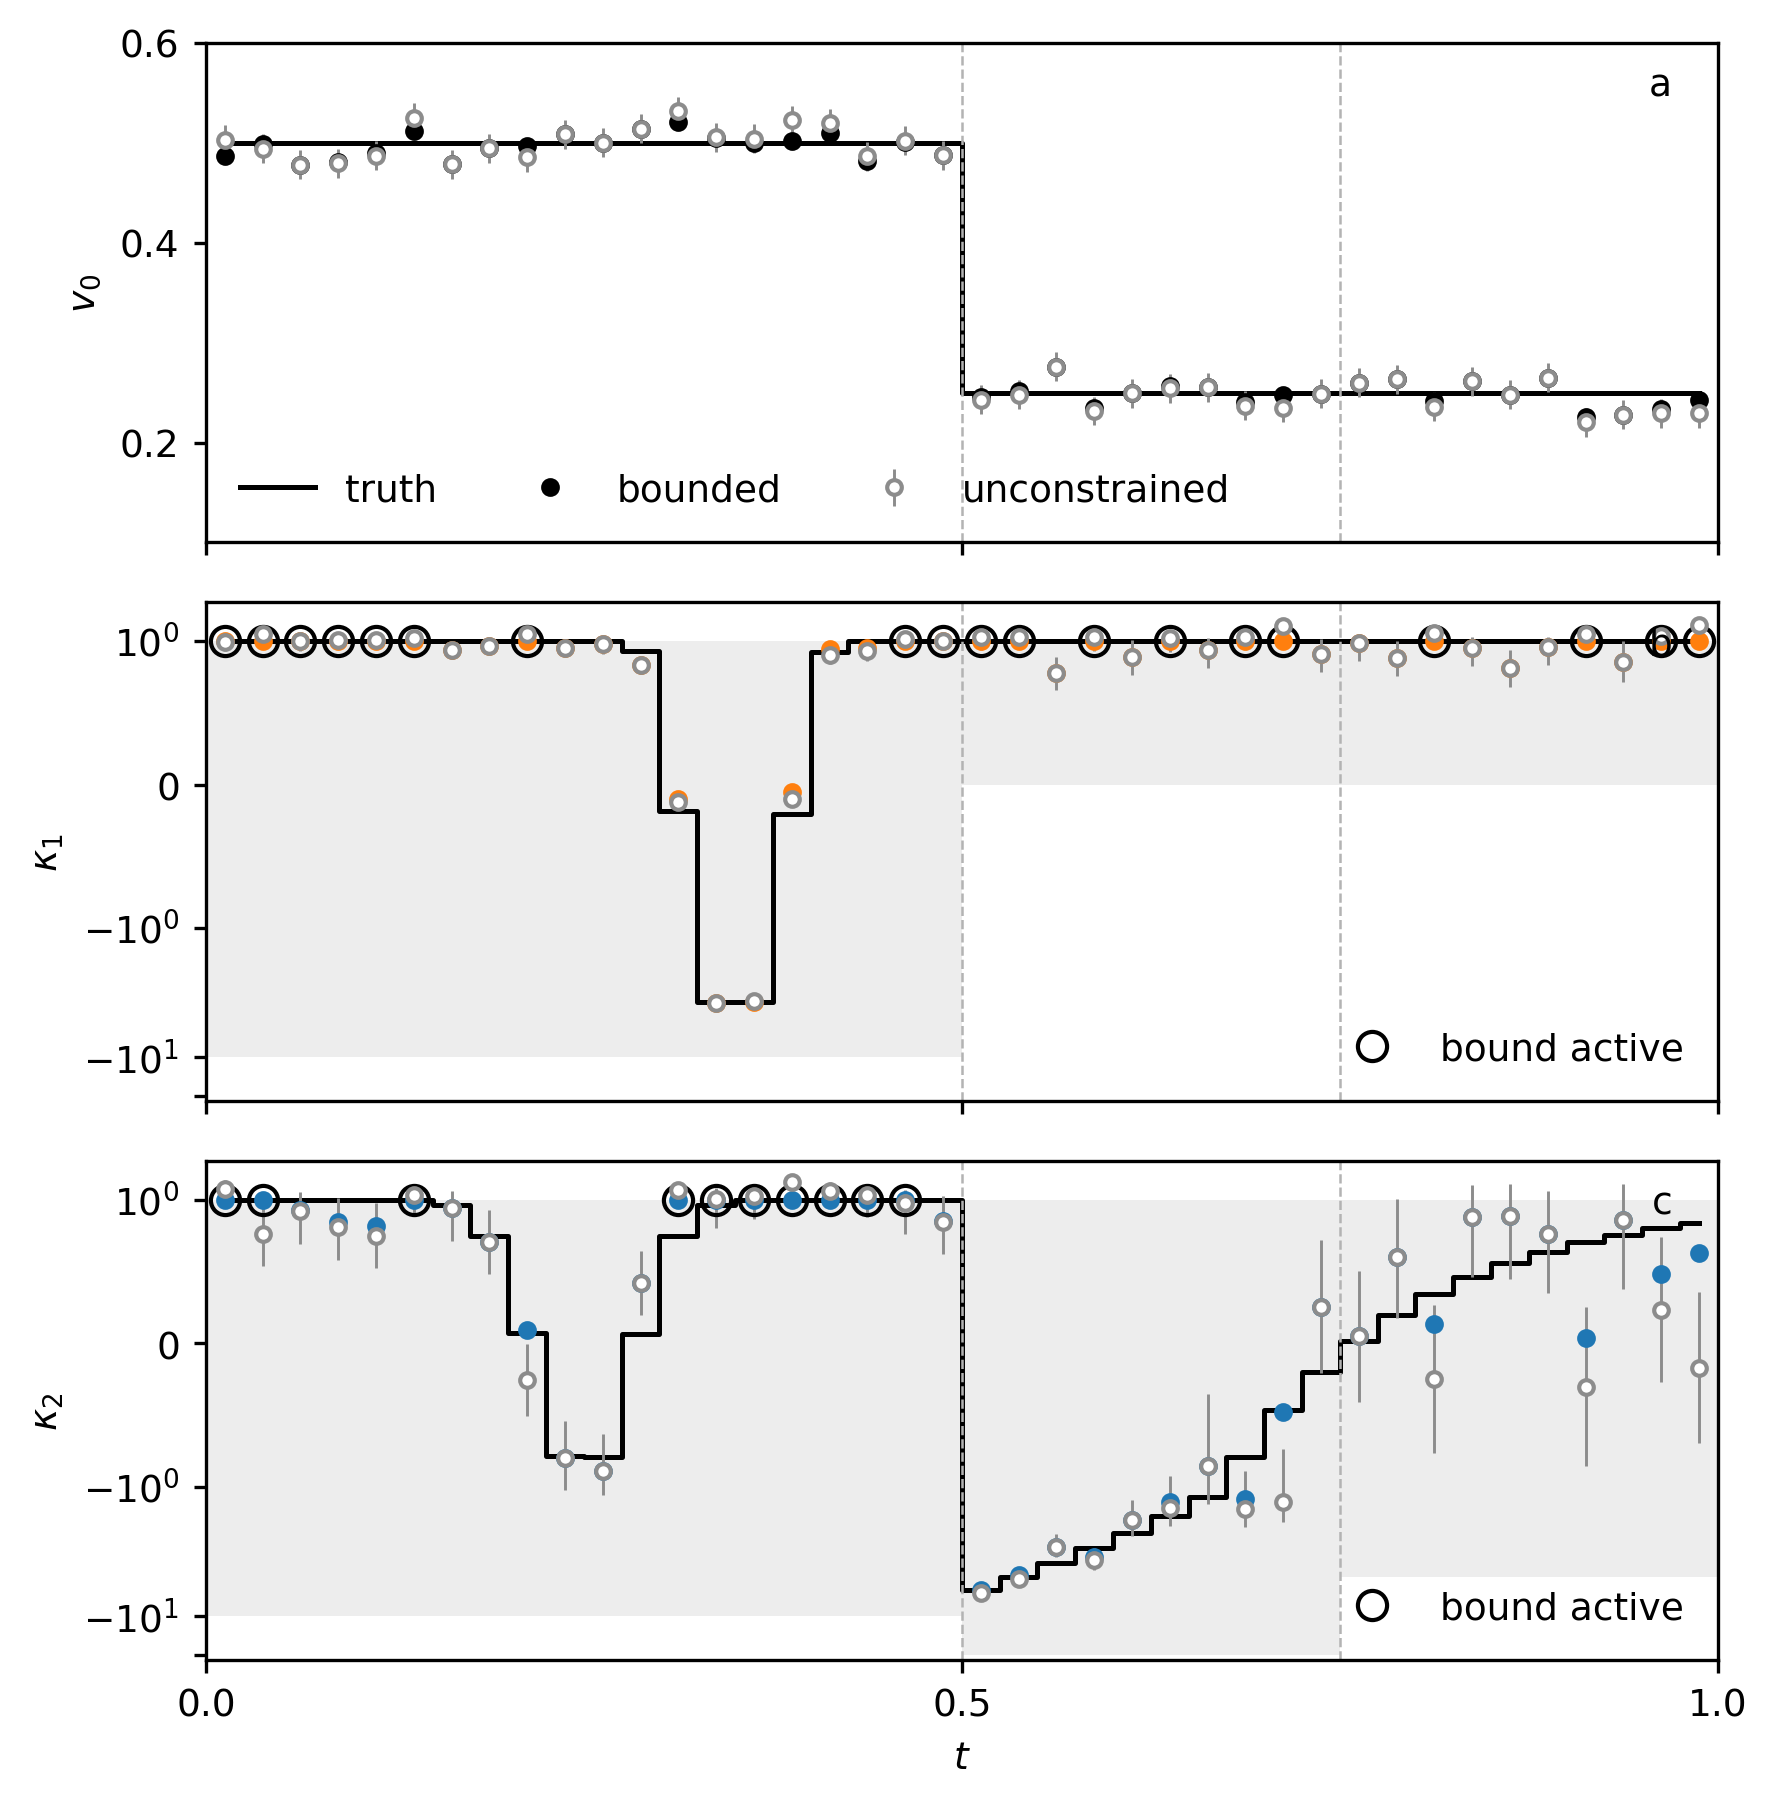
\includegraphics[width=0.8\textwidth]{fig2_per_epoch_bounded.png}
\caption{Independent per-epoch solves. Black step: epoch-mean truth. Open gray circles with error bars: unconstrained weighted least squares. Filled circles: bounded solution; large open circles mark epochs where a coupling bound is active. Shading: the known per-epoch bounds. Dashed lines: the earthquake and the bound change at $t = 0.75$.}
\label{fig:epochs}
\end{figure}

\FloatBarrier
\section{Structured priors from the known earthquake time}
\label{sec:priors}

The method applies four priors in sequence. Three are physics that follow from knowing when the earthquake occurred; the fourth is a generic robustness choice and is labeled as such.

\subsection{Prior 1: the block rate is piecewise constant between earthquakes}

Within each interseismic segment $\mathcal{S}$ the block rate is pooled by inverse-variance weighting of the per-epoch estimates,
\begin{equation}
\hat{v}_0^{\mathcal{S}} = \frac{\sum_{t \in \mathcal{S}} w_t\, v_{0,t}^\ast}{\sum_{t \in \mathcal{S}} w_t},
\qquad w_t = 1 / (\mat{\Sigma}_t)_{v_0 v_0},
\end{equation}
and every epoch is then re-solved with $v_0$ fixed at the pooled value. With $v_0$ known the coupling bounds are a plain box on $(e_1, e_2)$, so the re-solve is a bounded linear least-squares problem in two unknowns,
\begin{equation}
\hat{\vect{e}}_t = \argmin_{\vect{e}}\; \norm{\mat{W}_t^{1/2}\bigl(\mat{A}_e \vect{e} - (\vect{d}_t - \vect{a}_0 \hat{v}_0^{\mathcal{S}})\bigr)}^2
\quad\text{s.t.}\quad \kappa_{\mathrm{lo}}(t)\,\hat{v}_0^{\mathcal{S}} \le \vect{e} \le \kappa_{\mathrm{hi}}(t)\,\hat{v}_0^{\mathcal{S}}.
\end{equation}
This is where most of the improvement comes from. Block rate and slip deficit trade off strongly in the per-epoch solves (correlations near 0.9), so fixing the block rate tightens the slip-deficit estimates well beyond the reduction in block-rate error alone. Figure~\ref{fig:blockrate} shows the pooled block rate; its root-mean-square error against truth is 0.0015, compared with 0.0126 for the per-epoch estimates.

\begin{figure}[htbp]
\centering
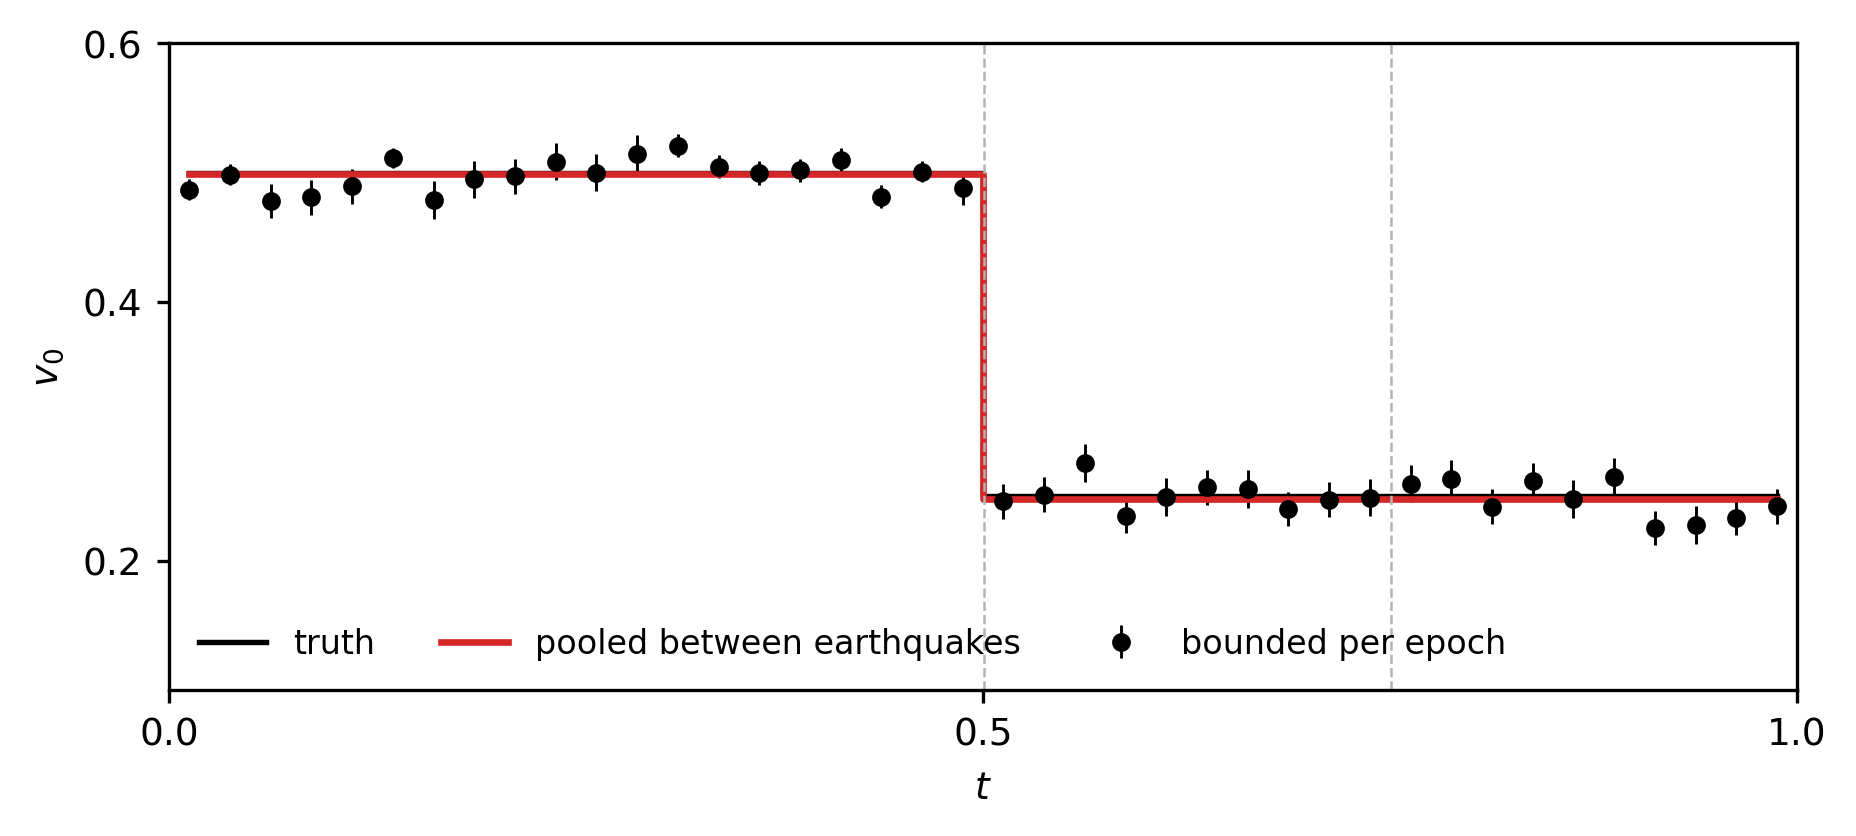
\includegraphics[width=0.8\textwidth]{fig7_block_rate_pooled.png}
\caption{Block rate per epoch (bounded solves, with one-sigma bars from the reduced covariance) and pooled between earthquakes.}
\label{fig:blockrate}
\end{figure}

\subsection{Prior 2: the temporal prior breaks only at the earthquake}

Deformation is expected to evolve smoothly except at the earthquake itself. The first-difference penalty used below therefore omits the single difference across the earthquake epoch and nothing else. A known change in the prescribed bounds, such as the tightening at $t = 0.75$, is a statement about what is admissible, not a physical regime change, and does not break the prior.

\subsection{Prior 3: postseismic coupling recovers monotonically and smoothly}

On any patch whose post-earthquake bounds admit afterslip, that is $\kappa_{\mathrm{lo}}(t) < 0$ after the earthquake, the coupling trajectory over the post-earthquake epochs is replaced by the solution of a bounded, monotone, curvature-penalized smoother:
\begin{equation}
\begin{aligned}
\min_{\vect{\kappa}}\quad & \sum_t w_t\,(\kappa_t - \hat{\kappa}_t)^2 + \lambda_2 \norm{\mat{D}_2^{(s)} \vect{\kappa}}^2 \\
\text{s.t.}\quad & \kappa_{t+1} \ge \kappa_t, \qquad \kappa_{\mathrm{lo}}(t) \le \kappa_t \le \kappa_{\mathrm{hi}}(t).
\end{aligned}
\label{eq:monotone}
\end{equation}
Two details matter, and both were found by getting them wrong first.

\paragraph{Curvature is penalized in log time.} $\mat{D}_2^{(s)}$ is the second-derivative operator on the non-uniform grid $s_t = \log(t - t_{\mathrm{eq}} + \tfrac{1}{2}\Delta t)$. An exponential or Omori-type recovery is nearly straight in log time, whereas in linear time its sharp start carries almost all of the curvature and a curvature penalty flattens exactly the part of the signal that is most diagnostic.

\paragraph{Pinned epochs are censored, not exact.} Under monotonicity, a single noisy epoch that touches the upper bound and is treated as exact forces every later epoch onto the bound. In \eqref{eq:monotone} pinned epochs therefore enter with $\hat{\kappa}_t$ at the bound and weight $w_t$ from the \emph{unconstrained} variance, the second reading of Section~1. The box constraint still holds at every epoch.

The smoothing parameter is $\lambda_2 = 10$ times the median weight; the solver is a trust-region method for the small quadratic program with the exact constant Hessian. The result tracks the truth to within about 0.1 in coupling from $-6.3$ just after the earthquake to $0.9$ at the end of the record (Figure~\ref{fig:linking}h).

\subsection{Prior 4 (generic): changes are penalized robustly}

Everywhere else the epochs are linked by a Tikhonov smoother on the logit of normalized coupling,
\begin{equation}
u_t = \frac{\hat{\kappa}_t - \kappa_{\mathrm{lo}}(t)}{\kappa_{\mathrm{hi}}(t) - \kappa_{\mathrm{lo}}(t)}, \qquad z_t = \logit u_t,
\qquad
\min_{\vect{z}} \sum_t w_t (z_t - \hat{z}_t)^2 + \lambda \sum_{t \notin \text{breaks}} \rho(z_{t+1} - z_t),
\end{equation}
with weights from the delta method, $w_t = [u_t(1-u_t)]^2 / \mathrm{Var}(u_t)$, and epochs at an active bound pinned (weight $10^6$ times the largest interior weight, then reported exactly at the bound). The logit metric is what removes the one-sided bias on locked patches: near a bound the delta-method weight of a noisy interior epoch collapses, so the pinned neighbors dominate, while epochs well inside the interval keep their full weight. Normalized coupling is also the quantity that remains comparable when the bounds change.

The penalty $\rho$ is Huber rather than quadratic, implemented by iteratively reweighted least squares with the knee at twice the median interior standard deviation in $z$. Small differences are smoothed as before; a large genuine change such as a slow slip onset is penalized only linearly and is not halved. This prior is not physics. It is the observation that a quadratic difference penalty cannot both suppress noise and preserve a two-epoch transient, whereas a robust one can do both approximately.

\FloatBarrier
\section{Results}

Figure~\ref{fig:linking} compares four ways of linking the same bounded epoch solutions. Figure~\ref{fig:locked} zooms on the locked shallow patch after the earthquake, where the truncation bias lives.

\begin{figure}[htbp]
\centering
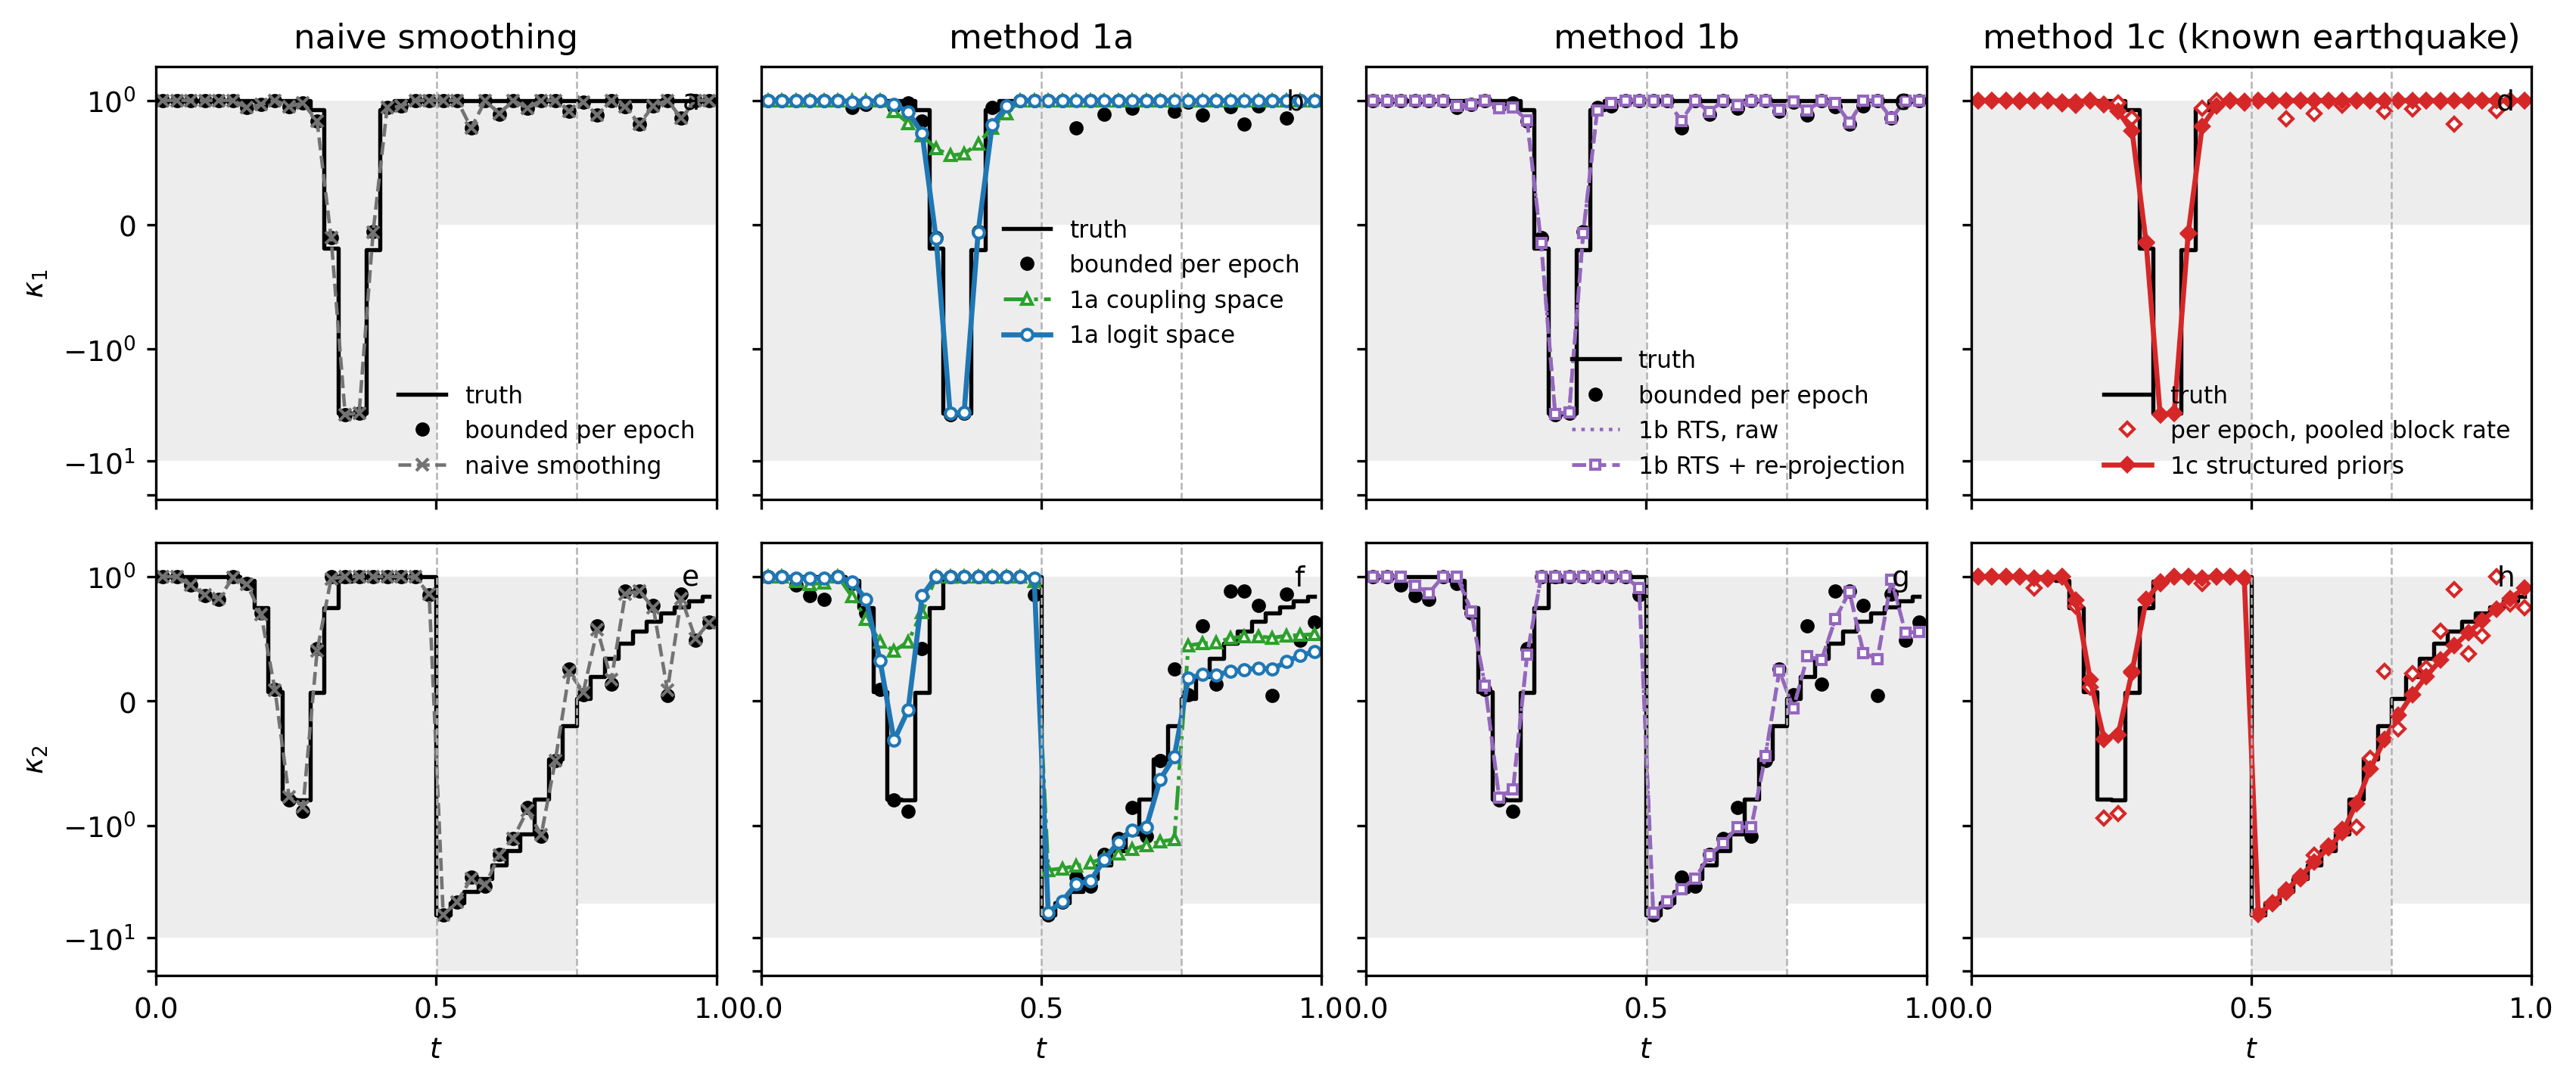
\includegraphics[width=\textwidth]{fig4_linking_methods.png}
\caption{Linking the epochs. Rows: shallow and deep patch coupling on a symmetric-log axis; black step is the epoch-mean truth; shading is the known bounds. Columns: naive smoothing of the bounded estimates; method 1a (normalized-coupling smoothing with pinned epochs, in coupling space and in logit space); method 1b (Rauch--Tung--Striebel fusion of the reduced covariances, before and after re-projection into the bounds); method 1c, the structured-prior method of this note (open diamonds: per-epoch estimates with the pooled block rate; filled diamonds and line: final estimate).}
\label{fig:linking}
\end{figure}

\begin{figure}[htbp]
\centering
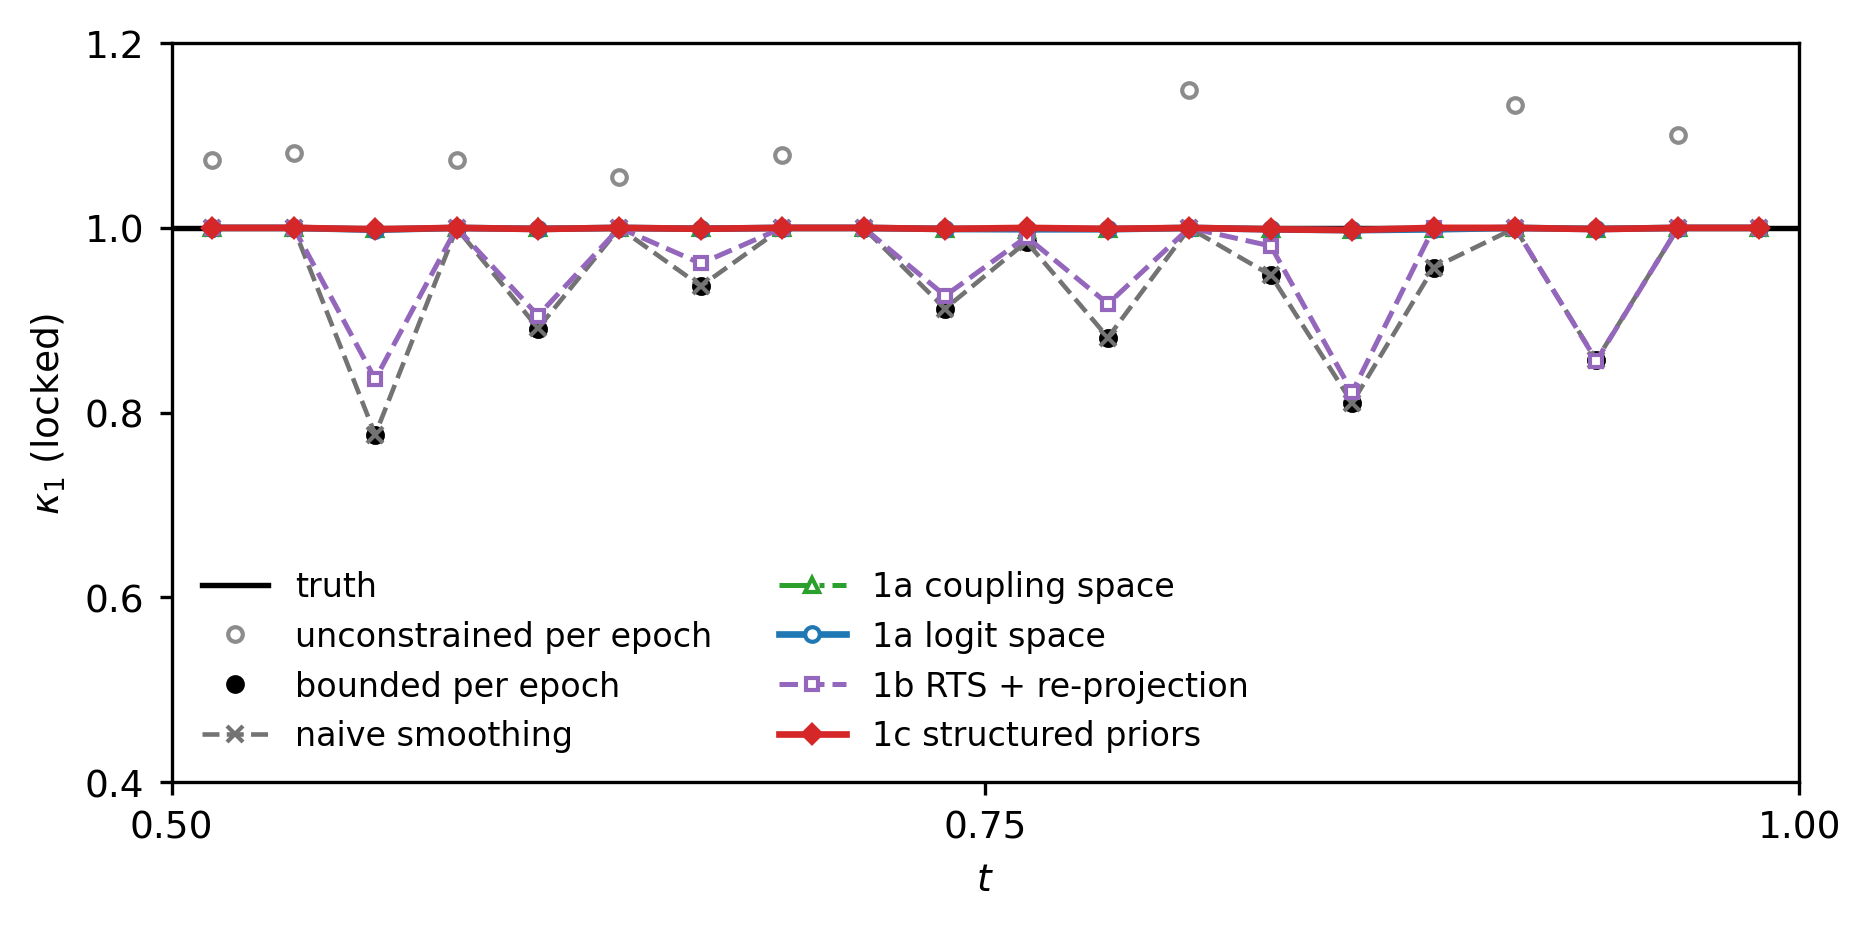
\includegraphics[width=0.85\textwidth]{fig3_fact_a_locked_patch.png}
\caption{The locked shallow patch after the earthquake. Unconstrained estimates scatter about 1; bounded estimates are one-sided with mean 0.948; naive smoothing inherits that bias. Methods that pin active-bound epochs (1a logit space, 1c) recover 1.000.}
\label{fig:locked}
\end{figure}

\begin{table}[htbp]
\centering
\small
\renewcommand{\arraystretch}{1.15}
\begin{tabular}{@{}lccc@{}}
\toprule
Method & RMSE $\kappa_1$ & RMSE $\kappa_2$ & mean $\kappa_1$, locked patch \\
\midrule
Unconstrained per epoch & 0.114 & 0.430 & 1.017 \\
Bounded per epoch & 0.072 & 0.294 & 0.948 \\
Naive smoothing of bounded & 0.071 & 0.273 & 0.948 \\
1a, logit-space Tikhonov & 0.050 & 0.287 & 0.999 \\
1b, RTS + re-projection & 0.061 & 0.185 & 0.960 \\
1c, per epoch with pooled block rate (prior 1 only) & 0.059 & 0.150 & 0.964 \\
\textbf{1c, structured priors (1 to 4)} & \textbf{0.049} & \textbf{0.134} & \textbf{0.999} \\
\midrule
Truth & & & 1.000 \\
\bottomrule
\end{tabular}
\caption{Root-mean-square error of coupling against the epoch-mean truth over all 40 epochs, and the mean estimate on the locked shallow patch after the earthquake (truth 1). Every final method satisfies the known bounds at every epoch on every patch; the unconstrained solve violates them in 26 of 80 patch-epochs.}
\label{tab:scores}
\end{table}

Three observations.

\begin{enumerate}
\item \textbf{Pooling the block rate is the single largest gain}, and it requires no smoothing at all. It cuts the deep-patch error in half before any temporal prior is applied. The mechanism is the strong trade-off between block rate and slip deficit in each epoch.
\item \textbf{Pinning active-bound epochs is what fixes the truncation bias}, and the logit metric is what lets the pinning propagate to noisy neighbors without smearing transients that sit well inside the bounds. Naive smoothing cannot recover the locked patch at any smoothing strength.
\item \textbf{The postseismic recovery is recovered essentially completely} once curvature is penalized in log time and pinned epochs are treated as censored. Both choices were necessary.
\end{enumerate}

\FloatBarrier
\section{Limitations and next steps}

The deep slow slip event before the earthquake is recovered to only about a third of its amplitude. It spans two epochs with a peak slip rate twice the plate rate, and any smoother whose kernel is wider than one epoch will shrink it; the robust penalty helps but does not eliminate the effect. Shorter epochs or an explicit change-point prior would address this; further tuning of $\lambda$ would not.

The smoothing parameters are fixed multiples of the median weight. Generalized cross-validation is unreliable here because pinned epochs are exact and dominate the criterion; the trade-off sweep in the script (figure 6) is the substitute, and it shows a broad plateau for the logit-space smoother between roughly 3 and 30 median weights.

The method as written is post-hoc: it never revisits the raw data and needs only the per-epoch point estimates, active sets, and sufficient statistics. That is what makes it cheap enough to run on a stack of existing runs. It is also its ceiling. A joint estimate that imposes these same priors while fitting all epochs at once would be the next step; the priors themselves, and the two lessons about log time and censoring, carry over unchanged.

For \code{celeri}, prior 1 corresponds to holding block rotations fixed within each interseismic segment and re-solving the mesh coefficients per epoch, which turns the bilinear coupling constraint into a linear one and removes the need for any iterative convexification. Prior 3 applies to any mesh whose post-earthquake bounds admit afterslip. Prior 2 and the censored treatment of pinned triangles apply everywhere.

\end{document}
